\clearpage
\section{Selective HDMI stimulation: 14 November 2026}
Resident image \texttt{c7531465}, MCU1803. Four PM data outputs were each
pulsed160 times independently: no SYS restart in32 completed trials. Eight
idle controls were also stable. SPI signatures were read with data outputs
held static zero. No PLL changes, output-enable release, direction reversal
or FPGA reload was performed.
\begin{center}\begin{tabular}{rrr}\toprule
SPI divider & Approximate SCK & Restarts / completed frames\\\midrule
60 & 1.002MHz & 8/16\\
600 & 100.197kHz & 3/9\\
6000 & 10.020kHz & 4/9\\
65535 & 917.34Hz & 5/9\\\bottomrule\end{tabular}\end{center}
One additional fast frame was interrupted by a read timeout; its raw trace is
retained and excluded from the completed denominator. A bounded repeat
completed. All returned signatures were correct. Two long-frame series each show5 restarts in9 reads. A busy sample preceding
a blocked counter read does not prove a reset during SEL assertion.
A timed repeat places nominal reset epochs around41--44ms after start,
about6--8ms after expected frame completion. This is read-completion time
minus fresh SYS uptime, assuming running clocks and small reply latency;
it is not a direct electrical latch. SEL deassertion remains a possible trigger.
Conservative analysis counts observed counter decreases only; original helper
host-time flags after delayed reads are superseded by raw recomputation.

SEL, SCK and MOSI remain coupled by the resident SPI master. These results
narrow the observed trigger to SPI traffic but do not establish an individual
faulty wire, MCU action or PLL cause. Polling does not exclude short OE/ready
or electrical glitches. MMCM LOCK is not directly recorded in this image.
Independent SPI pin control requires a gateware extension; Kasli was not
reloaded because its outputs are required to remain driven.

Final checks: original mode/divider restored, driven SPI retained, power
healthy, TDC frontend0xfff and a fresh physical ADC bankA capture passed
on all12 channels. Raw traces, executed sources and final ADC buffers:
\texttt{system/evidence-selective-20261114}.
\begin{figure}[htbp]\centering
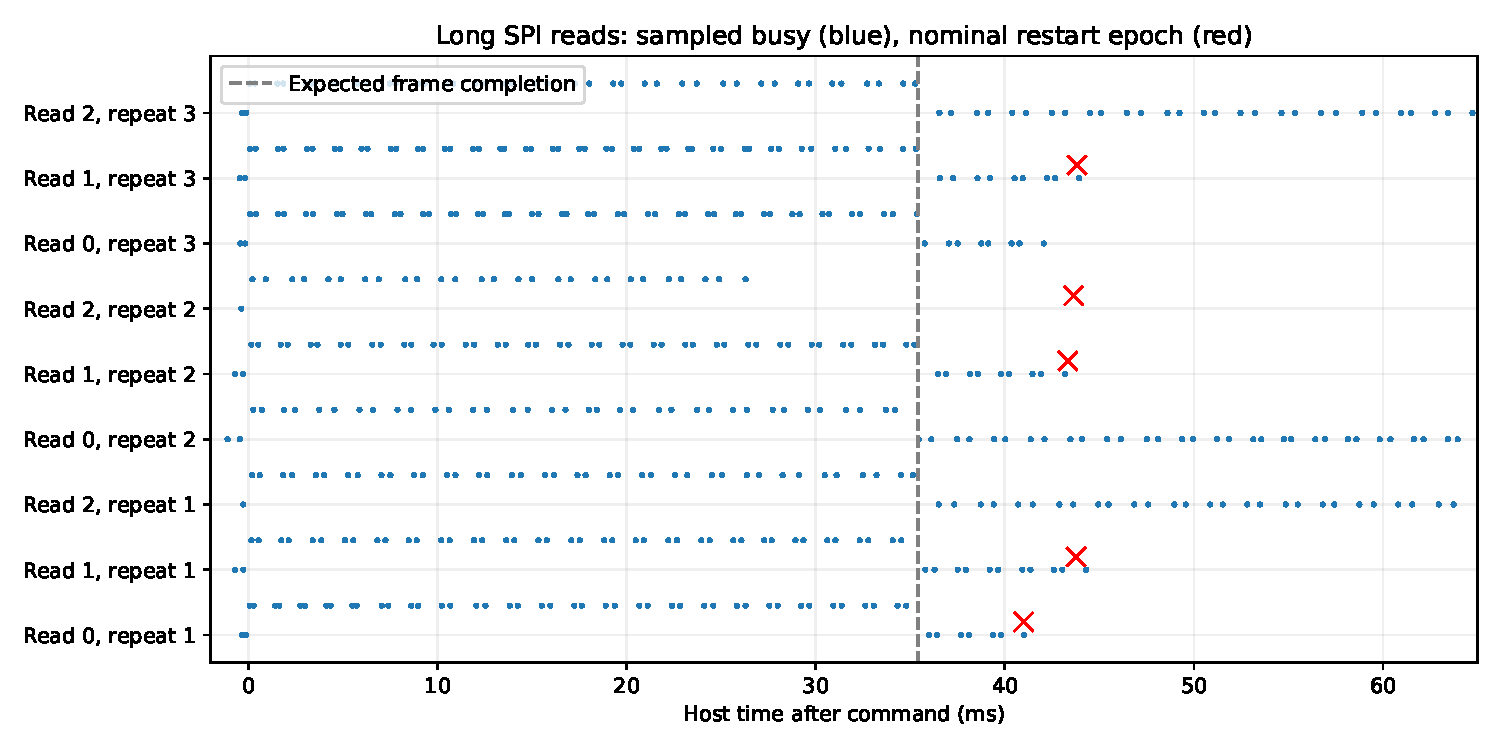
\includegraphics[width=\textwidth]{selective-spi.pdf}
\caption{Long SPI reads. Raised blue levels denote sampled master busy;
red crosses mark nominal reset epochs from fresh uptime. Host polling is not a
continuous electrical measurement.}
\end{figure}\clearpage
